\section{Silniki magazynu danych}
Niniejszy rozdział poświęcony jest omówieniu zagadnień związanych z silnikami bazy danych. Silnik bazy danych jest częścią bazy danych odpowiedzialną za wykonywanie kodu SQL, czyli wykonywanie operacji na danych. SQL jest językiem deklaratywnym. Klient, podając polecenie SQL, opisuje warunku, jakie musi spełnić końcowe rozwiązanie, a nie szczegółową implementację. Z tego wynika, że to silnik bazy danych odpowiedzialny jest za dostarczenie implementacji pozwalającej na wykonywanie kodu SQL. Silnik dodatkowo definiuje sposób przechowywania dnaych oraz zbiór operacji, które możemy na nich wykonać.

Architektura MySQL umożliwia korzystanie z wielu różnych silników. Silnik bazy danych wybierany jest per tabela, co oznacza, że w ramach pojedynczej bazy danych można używać różnych silników.
\subsection{Krótka charakterystyka podstawowych silników.}
W tym podrozdziale nie zostały przedstawione szczegółowe opisy silników dostępnych w MySQL, raczej ich główne charakterystyki, zalety oraz ograniczenia. Część z silników pominięto ze względu na ich marginalną popularność oraz zastosowanie. W zdecydowanej większości przypadków aktualnie najodpowiedniejszym silnikiem jest InnoDB, aczkolwiek każdy z silników opisanych w tym rozdziale ma pewne zalety. W tym podrozdziale sprawdzono, czy w pewnych sytuacjach zasadne jest użycie jednego z alternatywnych silników.
\subsubsection{MyISAM}
MyISAM był domyślnym silnikiem składowania danych do wersji 5.4 (włącznie). Każda tabela przechowywana jest w dwóch plikach na dysku twardym. Dane przechowywane są w pliku z rozszerzeniem \textbf{.MYD (MYData)}
natomiast w drugim pliku (\textbf{.MYI(MYIndex)}) składowane są indeksy. Poniżej przedstawiono kilka cech tego silnika bazy danych. 
\begin{itemize}
	\item \textbf{Brak wsparcia dla transakcji.} Z tego powodu MyISAM nie powinien być używany do tabel, dla których istotnym wymaganiem jest zapewnienie integralności danych.
	\item \textbf{Obsługa indeksów B-tree oraz Geospatial.}
	\item \textbf{Blokady tabeli.}  W momencie wykonywana operacji dodającej dane do tabeli jest ona blokowana na cały czas wykonywania operacji (również dla operacji odczytujących dane). Sprawia to, że w przypadku dużej liczby operacji modyfikujących dane - wydajność bazy danych wyraźnie spada.
	\item \textbf{Brak obłusgi mechanizmu kluczy obcych}
	\item \textbf{Mechanizm kompresji danych.} Silnik umożliwia kompresowanie danych w celu optymalizacji ilości miejsca potrzebnego do przechowywania danych z tabeli. Taka operacja sprawia, że skompresowane dane są dostępne jedynie do odczytu, a ich modyfikacja jest zablokowana i wymaga rozpakowania danych. Tabele MyISAM można kompresować i dekompresować za pomocą mechanizmu \textit{myisampack}.
	\item \textbf{Buforowanie indeksów.} Silnik MyISAM buforuje jedynie indeksy.
	\item \textbf{Obsługa statystyk.}
\end{itemize}

W czasie pisania tej pracy silnik MyISAM nie był już rozwijany, dlatego autor odradza jego stosowanie w nowszych wersjach serwera MySQL. 

\subsubsection{InnoDB}
Od wersji 5.5 InnoDB jest domyślnym silnikiem bazy danych MySQL. Mechanizm InnoDB uzupełniono o funkcje, których brakowało w MyISAM i obecnie jest zdecydowanie najpopularniejszym wyborem. Domyślnie dane przechowywane są w pojedynczych plikach, ale możliwe być również przechowywane w wielu plikach. Strukturę plików bazy \textit{StackOverflow}, która dla wszystkich tabel używa silnika InnoDB, przedstawiono na rysunku ~\ref{fig:innodb-fileslabel}.
\begin{figure}[!h]
	\caption{Pliki silnika InnoDB testowej bazy danych \textit{StackOverflow}}
	\centering
	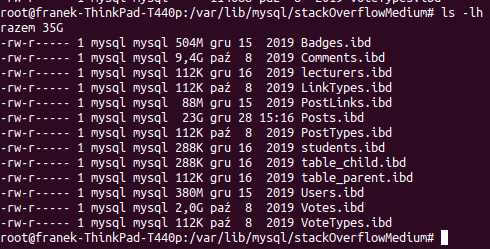
\includegraphics[scale = 0.43]{innodb-files.png}
	\label{fig:innodb-fileslabel}
\end{figure}
Poniżej przedstawiono podstawowe charakterystyki silnika.
\begin{itemize}
	\item \textbf{Wsparcie dla transakcji.} Silnik wspiera transakcje oraz wszystkie cztery poziomy izolacji modelu \textit{ANSI}. Poziom izolacji transakcji określa zasady widoczności pomiędzy współbieżnymi transakcjami. Dzięki wsparciu dla wszystkich czterech izolacji  silnik InnoDB spełnia wymagania stawiane aplikacją wymagającym zapewnienie integralności danych. 
	\item \textbf{Wsparcie dla indeksów.} InnoDb wspiera najważniejsze indeksy takie jak: B-tree, Hash, Spatial.
	\item \textbf{Blokowanie dostępu na poziomie rekordów. } Dostęp do tabel InnoDB jest blokowany za pomocą mechanizmy MVCC (Multi-Versioned Concurrency Control). Blokowane są pojedyncze rekordy, zamiast całej tabeli. Wprowadzenie tej zmiany znacząco zwiększyło wydajność równoległych operacji modyfikujących dane w tabeli.
	\item \textbf{Wsparcie dla kluczy obcych.}
	\item \textbf{Buforowanie danych oraz indeksów.} Silnik InnoDb może buforować nie tylko indeksy, ale również dane.
	\item  \textbf{Nieskompresowane indeksy.} Silnik InnoDb nie kompresuje indeksów, co prowadzi do zwiększenia zużycia przestrzeni dyskowej.
	\item \textbf{Wsparcie dla partycjonowania.} Szerzej opisane w podrozdziale dotyczącym partycjonowania.
	\item \textbf{Obsługa statystyk.}
\end{itemize}

\subsubsection{CSV Storage Engine}
Silnik CSV Storage Engine przechowuje dane tabeli w plikach tekstowych w formacie csv z wartościami rozdzielonymi przecinkami. Ten silnik może być przydatny, jeżeli chcemy nasze dane przechowywać w formacie csv. Posiada wiele ograniczeń, dlatego autor nie zaleca jego stosowania, o ile nie zależy nam na przechowywaniu danych tabeli w formacie CSV.
Poniżej przedstawiono podstawowe ograniczenia tego silnika.
\begin{itemize}
	\item \textbf{Brak wsparcia dla indeksów i kluczy obcych.}
	\item \textbf{Brak wsparcia dla transakcji.}
	\item \textbf{Brak możliwości przechowywania wartości \textit{null}.}
	\item \textbf{Brak wsparcia dla partycjonowania.}
\end{itemize}

\subsubsection{Memory}
Silnik Memory przechowuje wszystkie dane w pamięci, a nie na dysku twardym. Te dane są ulotne i zostają usunięte w momencie restartu serwera (struktura tabeli zostaje zachowana). Z powodu przechowywania w pamięci są o rząd wielkości szybsze od standardowych silników baz danych, ale ze względu na swoją ulotność nie powinny przechowywać istotnych danych dla aplikacji.
Poniżej przedstawiono podstawowe własności tabeli Memory.
\begin{itemize}
	\item \textbf{Wsparcie dla indeksów} Tabele Memory obsługują indeksy Hash oraz B-tree. Domyślnym indeksem jest indeks typ Hash.
	\item \textbf{Blokowanie na poziomie tabeli.} Podobnie jak tabele MyISAM, w momencie modyfikowania danych blokowana jest cała tabela.
	\item \textbf{Brak obsługi typów TEXT oraz BLOB}. Tabele nie obsługują typów TEXT. Przechowywanie teksu możliwe jest w kolumnach VARCHAR o stałej zdefiniowanej wielkości, co prowadzi do marnotrawienia pamięci.
	\item \textbf{Brak danych statystycznych indeksu.} Tabele MEMORY nie przechowują statystyk dotyczących indeksów, co czasami może skutkować wybraniem nieodpowiedniego indeksu przez optymalizator zapytań i w efekcie pogorszenie wydajności zapytań.
	\item \textbf{Brak wsparcia dla transakcji.}
\end{itemize}

Zastosowanie silnika MEMORY warto rozważyć w następujących sytuacjach.
\begin{itemize}
	\item Pamięć podręczna dla często odczytywanych danych, która jest wczytywana w momencie startu serwera.
	\item Buforowanie wyników agregowanych danych z często wykonywanych zapytań.
	\item Przechowywanie wyników pośrednich z zapytań.
	\item MySQL używa tabeli Memory do wewnętrznego przetwarzania zapytań wymagających tabeli tymczasowych do przechowywania wyników pośrednich.
\end{itemize}

\subsubsection{Silnik Archive}
Archive jest silnikiem służącym do przechowywania dużej ilości nieindeksowanych danych, które są rzadko pobierane. Jego głównym zastosowaniem jest archiwizacja danych z wysokim poziomem kompresji danych.

Podstawowe cechy tego silnika przedstawiono poniżej.
\begin{itemize}
	\item \textbf{Brak wsparcia dla transakcji.}
	\item \textbf{Możliwe wykonywanie jedynie operacji INSERT, REPLACE oraz SELECT}. W tabelach Archive niemożliwe jest usuwanie i modyfikowanie istniejących krotek.
	\item \textbf{Brak wsparcia dla indeksów.}
	\item \textbf{Blokowanie na poziomie tabeli.}
	\item \textbf{Kompresowanie danych.} Każdy wstawiony rekord jest automatycznie kompresowany za pomocą \textit{zlib}, dlatego tabele Archive wymagają zdecydowanie mniej miejsca od tabel InnoDB lub MyISAM.
\end{itemize}


\subsection{Porównanie silników}



\subsubsection{Przechowywanie danych}
W celu porównania sposobu przechowywania danych na dysku przegotowano testową bazę danych, zawierającą pięć tabel będących niemalże kopią tabeli \textit{Users} z bazy testowej, z których każda wykorzystuje inny silnik. Jedyną zmianą jest brak kolumny \textit{AboutMe}, która została usunięta ze względu brak wsparcia dla kolumn TEXT w silniku MEMORY. Do tworzenia tabel wykorzystano polecenia z poniższego listingu, a następnie zaimportowano dane z bazy \textit{Stackoverflow}. Ponieważ nie wszystkie silniki wspierają przechowywania wartości NULL, zamieniono domyślne wartości NULL na wartość 0 lub pusty tekst (w zależności od typu danych).
\begin{spverbatim}
	CREATE TABLE `Users` (
	`Id` INT NOT NULL,
	`Age` INT NOT NULL DEFAULT 0,
	`CreationDate` DATETIME NOT NULL,
	`DisplayName` VARCHAR(80) NOT NULL,
	`DownVotes` INT NOT NULL,
	`EmailHash` VARCHAR(80) NOT NULL DEFAULT '',
	`LastAccessDate` DATETIME NOT NULL,
	`Location` VARCHAR(200) NOT NULL DEFAULT '',
	`Reputation` INT NOT NULL,
	`UpVotes` INT NOT NULL,
	`Views` INT NOT NULL,
	`WebsiteUrl` VARCHAR(400) NOT NULL DEFAULT '',
	`AccountId` INT NOT NULL DEFAULT 0,
	PRIMARY KEY (`Id`) -- w tabelach, które wspierają klucze główne
	) ENGINE=<nazwa silnika>;
\end{spverbatim}
Klucze główne usunięto w przypadku silników, które ich nie wspierają. Ostatecznie tabela zawiera około 2,5 miliona wierszy.
\begin{figure}[!h]
	\caption{Baza danych użyta do testowania silników baz danych}
	\centering
	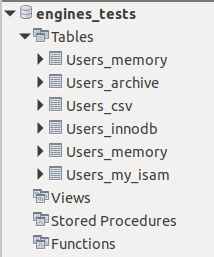
\includegraphics[scale = 0.7]{engines_tests.png}
	\label{fig:label}
\end{figure}
\begin{figure}[!h]
	\caption{Pliki z danymi użytkowników dla testowych silników.}
	\centering
	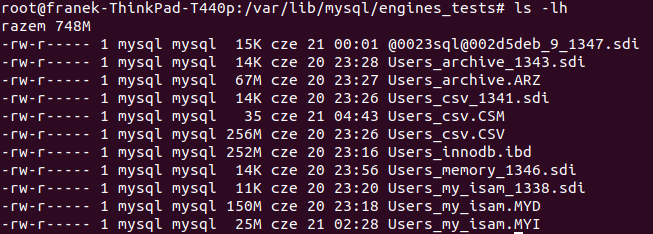
\includegraphics[scale = 0.7]{engines_storage.png}
	\label{fig:engines_storage}
\end{figure}

Na rysunku ~\ref{fig:engines_storage} przedstawiono pliki tabel testowej bazy danych. Pod względem optymalizacji ilości miejsca na dysku zdecydowanie najlepiej wypada silnik Archive, który potrzebuje jedynie 67 MB dla danych użytkowników. Na drugim miejscu pod tym względem plasuje się silnik MyISAM. Silniki InnoDB oraz CSV wymagają praktycznie takiej samej przestrzeni dyskowej; w granicach 250 MB. Silnik MEMORY na dysku twardym przechowuje jedynie strukturę tabeli, ale do sprawdzenia ilości użytej pamięci możemy użyć narzędzia \textit{MySQL Workbench}.
\begin{figure}[!h]
	\caption{Informacje dotyczące tabeli Users\textunderscore memory w \textit{MySQL Workbench}. \textit{StackOverflow}}
	\centering
	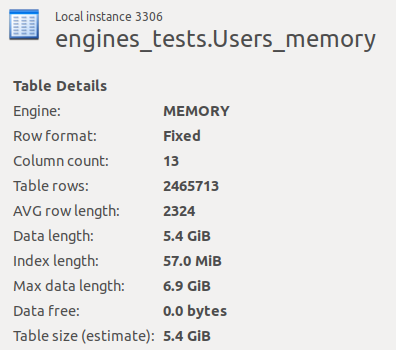
\includegraphics[scale = 0.6]{memory_engine_storage.png}
	\label{fig:label}
\end{figure}
Silnik MEMORY wymaga prawie 5.5 Gb pamięci. Wynika to w dużej mierze z tego, że silnik MEMORY dla kolumn VARCHAR zawsze rezerwuje rozmiar wynikający z maksymalnej wartości, nawet jeżeli nie jest ona wykorzystana.




\subsubsection{Wymaganie transakcyjności}
W przypadku tabel, które wymagają użycia transakcji, jedynym możliwym wyborem jest silnik InnoDB.

\subsubsection{Operacje odczytu klucz-wartość}
Do testowania użyto narzędzia \textit{sysbench}, które posiada wbudowany mechanizm ułatwiający testowanie baz danych. Za pomocą poniższych poleceń rzygotowano testową bazę danych udostępnioną przez \textit{sysbench}. 
\begin{spverbatim}
	sysbench --db-driver=mysql --mysql-user=root --mysql-password=root --mysql-db=test --table_size=2000000 --range_selects=off --mysql_storage_engine=
	<nazwa silnika> /usr/share/sysbench/oltp_read_only.lua prepare
\end{spverbatim} 
Baza danych zawiera 2 miliony rekordów, tabela domyślnie przyjmuje nazwę \textit{sbtest1}.
\begin{figure}[H]
	\caption{Struktura tabeli \textit{sbtest1}.}
	\centering
	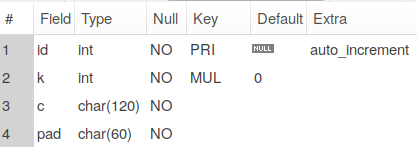
\includegraphics[scale = 0.6]{struktura_sbtest1.png}
	\label{fig:label}
\end{figure}

Aby wykonać test polecenie \textit{prepare} należy zamienić na polecenie \textit{run}. Przy takiej konfiguracji wykonywane jest następujące zapytanie:
\begin{spverbatim}
	SELECT c FROM sbtest1 WHERE id=?
\end{spverbatim}
\begin{figure}[H]
	\caption{Przykładowe statystyki testu wydajności izolowanych operacji odczytu.}
	\centering
	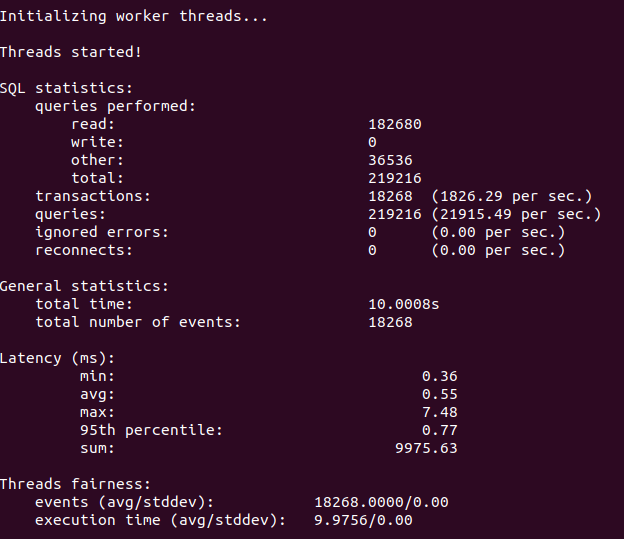
\includegraphics[scale = 0.6]{sysbench_statistics.png}
	\label{fig:label}
\end{figure}
\begin{center}
	\begin{tabular}{ | c | c | c | c | c | c |}
		\hline
		- & MyISAM & InnoDB & Memory & Archive & CSV  \\ 
		\hline
		średni czas [ms] & 0.54 & 0.55 & 0.38 & powyżej minuty & powyżej minuty \\
		\hline
	\end{tabular}
\end{center}
Z powyższej tabeli wynika, że w przypadku zapytań używających pełnego klucza głównego, silnik MEMORY jest najwydajniejszy. Dobry wynik wynika z faktu zastosowania indeksu HASH na kolumnie Id. Silniki InnoDB oraz MyISAM prezentują podobną wydajność w przypadku zapytań używających indeksy (w tym przypadku indeksy BTree). Silniki Archive oraz CSV wyraźnie odstają w tym zestawieniu ze względu na brak obsługi kluczy głównych.


\subsubsection{Symultaniczne operacje odczytu z wykorzystaniem klucza głównego oraz operacji zapisu.}

Do przygotowania testowych zestawów danych wykorzystano następujące skrypty:
\begin{spverbatim}
	sysbench --db-driver=mysql --mysql-user=root --mysql-password=root
	--mysql-db=test --table_size=2000000 --num-threads=12
	--range_selects=off --mysql_storage_engine=<nazwa silinika>
	/usr/share/sysbench/oltp_read_write.lua prepare
\end{spverbatim}

Wykonanie testu analogicznie jak w poprzednich przypadkach wykonano, zamieniając słowo kluczowe \textit{prepare} na \textit{run}.


Na rysunku ~\ref{fig:wyniki_testu_symulatnicznych_odczytow} przedstawiono wyniki testu. W przypadku tego testu operacje odczytu wykonywane były równolegle z operacjami zapisu do tabeli.
\begin{figure}[H]
	\caption{Przykładowe statystyki testu symultanicznych odczytów i zapisów.}
	\centering
	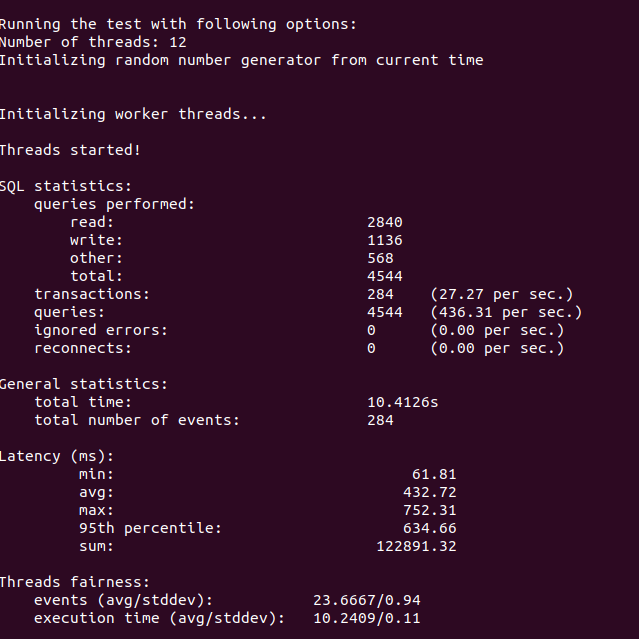
\includegraphics[scale = 0.6]{wyniki_testu_symulatnicznych_odczytow.png}
	\label{fig:wyniki_testu_symulatnicznych_odczytow}
\end{figure}
\begin{center}
	\begin{tabular}{ | c | c | c | c | c | c |}
		\hline
		- & MyISAM & InnoDB & Memory & Archive & CSV  \\ 
		\hline
		średni czas [ms] & 432.7 & 75.5 & 425.1 & powyżej minuty & powyżej minuty \\
		\hline
	\end{tabular}
\end{center}
Wyniki testu przedstawione w tabeli powyżej wskazują, że najwydajniejszym silnikiem w przypadku równoległych operacji odczytu i modyfikacji danych w środowisku wielowątkowym okazał się silnik InnoDB, na co wpływ ma zastosowanie mechanizmu blokowania pojedynczych rekordów, zamiast całej tabeli zastosowany w pozostałych.

\subsubsection{Wyszukiwanie danych z zakresu.}
Kolejny test symuluje operację wyszukiwania danych za pomocą zakresu. Do jego przygotowania wykorzystano następujące polecenie.
\begin{spverbatim}
	sysbench --db-driver=mysql --mysql-user=root --mysql-password=root
	--mysql-db=test --table_size=2000000 --mysql_storage_engine=<nazwa silniku>
	--num-threads=12 /usr/share/sysbench/select_random_ranges.lua prepare
\end{spverbatim}
W związku z tym, że domyślnym indeksem dla tabeli MEMORY jest indeks HASH, a nie B-tree, na tej tabeli dodatkowo utworzono indeks typu B-Tree, wykorzystując następujące polecenie.
\begin{spverbatim}
	CREATE INDEX k_12 on sbtest1(k) USING btree;
\end{spverbatim}
\begin{center}
	\begin{tabular}{ | c | c | c | c | c | c |}
		\hline
		- & MyISAM & InnoDB & Memory & Archive & CSV  \\ 
		\hline
		średni czas [ms] & 1.23 & 1.25 & 0.51 & 26687 & 51400 \\
		\hline
	\end{tabular}
\end{center}

Wyniki testu pokazują, że przy tego typu operacjach najwydajniejsze są silniki wykorzystujące indeksy typu B-Tree, które pozwalają w optymalny sposób wyszukiwać za pomocą zakresu. Silnik \textit{MEMORY} okazał się najszybszy ze względu na przechowywanie danych bezpośrednio w pamięci.

\subsubsection{Operacje zapisu.}
Kolejny test prezentuje wydajność operacji zapisu w środowisku wielowątkowym. Do jego wykonania użyto następującego polecenia:
\begin{spverbatim}
	 sysbench --db-driver=mysql --mysql-user=root --mysql-password=root
	 --mysql-db=test --table_size=2000000 --mysql_storage_engine=<nazwa silnika>
	 --num-threads=12 /usr/share/sysbench/oltp_insert.lua prepare
\end{spverbatim}

Wyniki testu przedstawiono w poniższej tabeli:
\begin{center}
	\begin{tabular}{ | c | c | c | c | c | c |}
		\hline
		- & MyISAM & InnoDB & Memory & Archive & CSV  \\ 
		\hline
		średni czas [ms] & 107.8 & 37.9 & 104.1 & 17.1 & 108.9 \\
		\hline
	\end{tabular}
\end{center}

W teście najszybszy okazał się silnik \textit{Archive}, który został zaprojektowany właśnie do wydajnego zapisywania danych. Znaczny wpływ na dużą wydajność ma fakt braku indeksów. Dzięki temu serwer nie spędza dodatkowego czasu na aktualizacji indeksu podczas wstawiania nowych krotek. Istotna jest również niemal trzykrotnie większej wydajność operacji zapisu w tabelach \textit{InnoDB} w porównaniu do \textit{MyISAM} i \textit{MEMORY}. Jest to wynikiem zastosowania blokowania na poziomie rekordu.

\subsubsection{Operacje aktualizacji danych z wykorzystaniem indeksu.}

Kolejny test przedstawia wydajność operacji aktualizacji danych z wykorzystaniem indeksu w środowisku wielowątkowym. Do jego przygotowania użyto następującego polecenia.
\begin{spverbatim}
	sysbench --db-driver=mysql --mysql-user=root --mysql-password=root 
	--mysql-db=test --table_size=2000000 --num-threads=12 
	--mysql-storage_engine=	<nazwa silnika> 
	/usr/share/sysbench/oltp_update_index.lua prepare
\end{spverbatim}

Wyniki testu zamieszczono w poniższej tabeli.
\begin{center}
	\begin{tabular}{ | c | c | c | c | c | c |}
		\hline
		- & MyISAM & InnoDB & Memory & Archive & CSV  \\ 
		\hline
		średni czas [ms] & 109.1 & 54.9 & 105.9 & Brak wsparcia & Brak indeksów \\
		\hline
	\end{tabular}
\end{center}

Test jest miarodajny jedynie dla trzech silników wspierających indeksy. Podstawową przyczyną powodującą niemal dwukrotnie większą wydajność operacji modyfikujących dane w silniku \textit{InnoDB}, jest mechanizm blokowania na poziomie rekordów.

\subsubsection{Operacje aktualizacji danych bez wykorzystania indeksów.}
Kolejny test również przedstawia wydajność operacji aktualizacji danych w środowisku wielowątkowym, ale bez wykorzystania indeksów.
Do wykonania testu użyto polecenia:
\begin{spverbatim}
	sysbench --db-driver=mysql --mysql-user=root --mysql-password=root
	--mysql-db=test --table_size=2000000 --num-threads=12 
	--mysql-storage_engine=	<nazwa silnika>
	/usr/share/sysbench/oltp_update_non_index.lua prepare
	
\end{spverbatim}
\begin{center}
	\begin{tabular}{ | c | c | c | c | c | c |}
		\hline
		- & MyISAM & InnoDB & Memory & Archive & CSV  \\ 
		\hline
		średni czas [ms] & 107.6 & 46.9 & 107.1 & Brak wsparcia & 67627.1 \\
		\hline
	\end{tabular}
\end{center}

Testy potwierdzają, że w środowisku wielowątkowym przy operacjach modyfikujących dane najwydajniejszy jest silnik \textit{InnoDB}, dzięki blokowaniu na poziomie rekordów.
\subsubsection{Operacje usuwania danych}
W kolejnym teście sprawdzono wydajność operacji usuwania danych w środowisku wielowątkowym.
\begin{spverbatim}
	sysbench --db-driver=mysql --mysql-user=root --mysql-password=root 
	--mysql-db=test --table_size=2000000 --num-threads=12 
	--mysql-storage_engine=<nazwa tabeli>  
	/usr/share/sysbench/oltp_delete.lua prepare
\end{spverbatim}

\begin{center}
\begin{tabular}{ | c | c | c | c | c | c |}
	\hline
	- & MyISAM & InnoDB & Memory & Archive & CSV  \\ 
	\hline
	średni czas [ms] & 312.5 & 43.3 & 106.1 & Brak wsparcia & 62342.1 \\
	\hline
\end{tabular}
\end{center}


Silnik InnoDB jest najwydajniejszym rozwiązaniem ze względu na mechanizm blokowania na poziomie rekordów.



\subsection{Podsumowanie}

W tym rozdziale przedstawiono podstawowe własności najpopularniejszych dostępnych obecnie silników MySQL. W zdecydowanej większości przypadków, które możemy spotkać we współczesnych aplikacjach, korzystających z baz danych najlepszym rozwiązaniem jest silnik InnoDB. W przypadku tabel, do których dane są jedynie zapisywane, ale nie odczytywane, dobrym wyborem jest silnik \textit{Archive}, który zapewnia najlepszą wydajność operacji zapisu, oraz zdecydowanie niższe zużycie przestrzeni dyskowej od pozostałych silników. Wyniki testów wydajnościowych potwierdzają, że silnik \textit{MyISAM} nie powinien być obecnie stosowany. Silnik \textit{InnoDB} będący jego następcą jest bardziej wydajny, a dodatkowo zawiera mechanizmy, których brakuje \textit{MyISAM}. Silnik \textit{MEMORY} w środowisku wielowątkowym nie jest bardziej wydajny od \textit{InnoDB}, a dodatkowo zużywa wiele pamięci. Silnik \textit{CSV} jest niewydajny i ubogi w funkcje, dlatego według autora nie powinien być używany w produkcyjnych zastosowaniach.